\begin{figure}
    \centering
    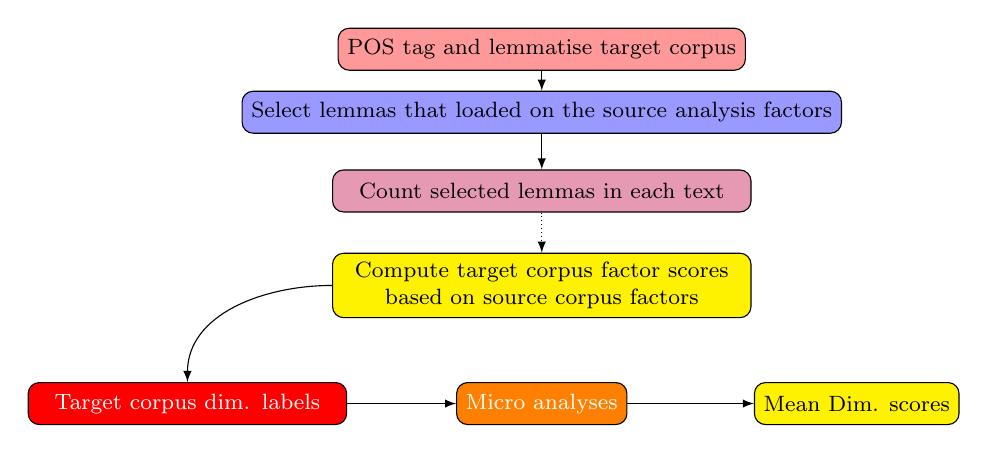
\begin{tikzpicture}
        %\tikzstyle{block} = [rectangle, rounded corners, text=black, text centered, draw=black, minimum height=.3in]
        \tikzstyle{block} = [rectangle, rounded corners, text=black, text centered, draw=black,font=\footnotesize, minimum height=.21in]
        \tikzstyle{line} = [-latex,draw=black,line width=.4]
        \node[block,fill=red!40,text=black] (tag) at (5,3) {POS tag and lemmatise target corpus};
        \node[block,fill=blue!40,text=black] (norm) at (5,2.2) {Select lemmas that loaded on the source analysis factors};
        \node[block,fill=purple!40,text=black, text width=2in] (selectvars) at (5,1.2) {Count selected lemmas in each text};
        %\node[block,fill=blue!40,text=black, text width=1.5in] (count) at (3,.3) {Target corpus Count $x$};
        %\node[block,fill=blue!40,text=black, text width=1.5in] (mean) at (3,-.3) {Source corpus Mean $\mu$};
        %\node[block,fill=blue!40,text=black, text width=1.5in] (std) at (3,-.9) {Source corpus STD $\sigma$};
        %\node[block,fill=blue!40,text=black] (comm) at (1,-.2) {Commun.};
        %\node[block,fill=green!40,text=black,align=center] (zscore) at (8,-.3) {Target \\ Z-Score \\ \( z = \frac{{x - \mu}}{{\sigma}} \)};
        %\node[block,fill=green!40,text=black] (load) at (7,-.2) {Drop weak loadings};
        %\node[block,fill=green!40,text=black] (standard) at (7,-1) {Standardise counts};
        \node[block,fill=yellow,text=black, text width=2in] (scores) at (5,0) {Compute target corpus factor scores based on source corpus factors};
        \node[block,fill=red,text=white, text width=1.5in] (labels) at (.5,-1.5) {Target corpus dim. labels};
        \node[block,fill=orange,text=white] (analyse) at (5,-1.5) {Micro analyses};
        \node[block,fill=yellow,text=black] (dimscores) at (9,-1.5) {Mean Dim. scores};
        \draw[line] (tag) to (norm);
        \draw[line] (norm) to (selectvars);
        \draw[line, densely dotted] (selectvars) to[in=90,out=270] (scores);
        \draw[line] (scores) to[in=90,out=180] (labels);
        \draw[line] (labels) to (analyse);
        \draw[line] (analyse) to (dimscores);
        %\draw[line] (analyse) to[in=180,out=180,looseness=2.5] (dimscores);
        %\draw[line] (zscore) to[out=180,in=90] (0,-1.5) to[out=270,in=180] (scores);
    \end{tikzpicture}
    \caption{Additive Lexical Multi-Dimensional Analysis \citep{biberVariationEnglishMultiDimensional2001, berbersardinhaAddingRegistersPrevious2019}}
    \label{fig:additive_lexical_md_analysis}
\end{figure}
